\section{Optimal Capacity Expansion - Whats the Problem?}

\subsection{Peak load Pricing}

\begin{frame}
\frametitle{How much capacity is optimal?}
\begin{columns}
\begin{column} {0.4\textwidth}

\begin{figure}[h]
\centering
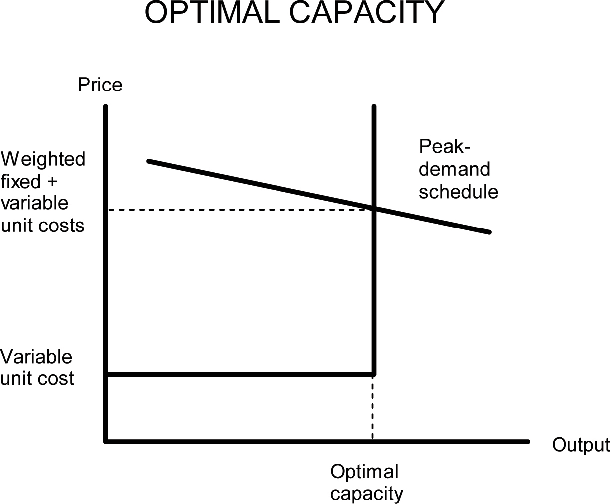
\includegraphics[width=1.\textwidth]{capacity/peak_load_opt}
    \caption{von der Fehr and Harbord (1997)}
    \label{fig:Daten 2004}            
\end{figure}
\end{column}

\begin{column} {0.6\textwidth}
\begin{itemize}
\item Optimal Capacity should be set such as to equate marginal benefits and costs from one unit of capacity
\end {itemize}
  
\begin{equation}
	c=(p^p-v)*v
\end{equation}

\begin{itemize}
\item Which is exactly what a perfectly competitive firm would do
\end {itemize}

\end{column}
\end{columns}
	

\end{frame}